\documentclass[conference]{IEEEtran}
\IEEEoverridecommandlockouts
% The preceding line is only needed to identify funding in the first footnote. If that is unneeded, please comment it out.
\usepackage{cite}
\usepackage{amsmath,amssymb,amsfonts}
\usepackage{cite}
\usepackage{algpseudocode}
\usepackage{graphicx}
\usepackage{textcomp}
\usepackage{xcolor}
\usepackage{amsthm}
\usepackage{algorithm}
%\usepackage{algorithmic}
\usepackage{epstopdf}
\usepackage{subfigure}
\usepackage{verbatim}
\usepackage{diagbox}



\newcommand{\tabincell}[2]{\begin{tabular}{@{}#1@{}}#2\end{tabular}}
\def\BibTeX{{\rm B\kern-.05em{\sc i\kern-.025em b}\kern-.08em
    T\kern-.1667em\lower.7ex\hbox{E}\kern-.125emX}}
\begin{document}

\title{HTS:Research on Task Scheduling Technology for Heterogeneous Storage\\
{\footnotesize \textsuperscript{*}Note: Sub-titles are not captured in Xplore and
should not be used}
\thanks{Identify applicable funding agency here. If none, delete this.}
}

\author{\IEEEauthorblockN{1\textsuperscript{st} Given Name Surname}
\IEEEauthorblockA{\textit{dept. name of organization (of Aff.)} \\
\textit{name of organization (of Aff.)}\\
City, Country \\
email address}
\and
\IEEEauthorblockN{2\textsuperscript{nd} Given Name Surname}
\IEEEauthorblockA{\textit{dept. name of organization (of Aff.)} \\
\textit{name of organization (of Aff.)}\\
City, Country \\
email address}
\and
\IEEEauthorblockN{3\textsuperscript{rd} Given Name Surname}
\IEEEauthorblockA{\textit{dept. name of organization (of Aff.)} \\
\textit{name of organization (of Aff.)}\\
City, Country \\
email address}
\and
\IEEEauthorblockN{4\textsuperscript{th} Given Name Surname}
\IEEEauthorblockA{\textit{dept. name of organization (of Aff.)} \\
\textit{name of organization (of Aff.)}\\
City, Country \\
email address}
\and
\IEEEauthorblockN{5\textsuperscript{th} Given Name Surname}
\IEEEauthorblockA{\textit{dept. name of organization (of Aff.)} \\
\textit{name of organization (of Aff.)}\\
City, Country \\
email address}
\and
\IEEEauthorblockN{6\textsuperscript{th} Given Name Surname}
\IEEEauthorblockA{\textit{dept. name of organization (of Aff.)} \\
\textit{name of organization (of Aff.)}\\
City, Country \\
email address}
}

\maketitle

\begin{abstract}
Nowadays, a trend in data center is that there are more and more heterogeneous storage devices, i.e. SSD and HDD, which may differ greatly in performance. However, data processing frameworks such as MapReduce often considers that hardware is homogeneous and task scheduling is not aware of the difference between heterogeneous storage devices. In this case, if a large number of tasks are scheduled on low-speed storage nodes, it will greatly cause data processing bottlenecks. Furthermore, due to the different performance of each disk, it is difficult to make all disks have the balanced load. In this paper, we formulate the above problem as Heterogeneous Storage-aware Task Scheduling Problem (HTS), and show its NP-hardness. In order to solve this problem, we propose a heuristic algorithm and a random algorithm whose distance from the optimum value is within $t$ with high probability. Experiments show that the our algorithm can reduce the task execution by up to 55\% over the storage-unaware scheduling mechanism.
\end{abstract}

\begin{IEEEkeywords}
big data processing, heterogeneous storage, task scheduling
\end{IEEEkeywords}

\section{Introduction}

Nowadays, in data centers that support big data processing platforms, i.e. Hadoop\cite{b14} and Spark\cite{b15}, there are more and more heterogeneous devices. On the one hand, due to the purchase of hardware devices from different hardware providers, such as Seagate\cite{b16} and Samsung\cite{b17}, the different standard hardware  lead to heterogeneous; on the other hand, the use and maintenance of equipment may also lead to heterogeneous. However, the underlying heterogeneity of devices is often neglected in big data platforms, which results in the mismatch between upper software and lower hardware. The result is a waste of hardware resources or low performance of big data processing.

In order to improve the performance of big data processing, we focus on heterogeneous storage devices. A data processing workload, named a job, are usually divided into parallel tasks which scheduled on each node for execution. A task execution is usually divided into two parts, the first part is the data reading stage, and the other part is the task execution stage. On the one hand, the speed of the processor is much faster than the I/O, on the other hand, the node usually has multiple processors. The above two aspects lead to that data reading stage will be the bottleneck of task execution, i.e. in TABLE \ref{tab1}. However, there are greatly differences in read performance between heterogeneous disks. Therefore, what we need to do is to select high-speed and low-load disks (If there are a large amount of tasks reading data on a high-speed disk at the same time, it may also cause bottlenecks in task execution) for tasks as much as possible. 

However, there are two aspects which make it difficult to solve the problem.
On the one hand, due to the different performance of heterogeneous disks, the same task might have different loads to the different disks. For example, the latency of read the same data $m_i$ from DISK-1 and DISK-2 are 0.3s and 0.1s, respectively. If task $t_i$ selects reading the data in DISK-1, the load to disk is 0.3 and selects DISK-2 is 0.1. On the other hand, because the data has been deployed on different disks before the task arrives, the task can only read data from fixed disks. For example, for HDFS data storage strategy, the redundancy factor of the data $m_i$ is 3, when a task needs to read the data $m_i$, only the 3 disks storing replica of $m_i$ can be selected. To avoid the bottleneck of reading during task execution, what we need to do is to balance the load of all disks. But the above two aspects make it difficult.
%On the other hand, because the data has been deployed on different disks before the task arrives, the task can only read data from fixed disks. For example, for HDFS data storage strategy, the redundancy factor of the data $m_i$ is 3, when a task needs to read the data $m_i$, only the 3 disks storing replica of $m_i$ can be selected. 从固定的几个选择,表明不能使得全局负载均衡

%Most of the previous work focused on data locality\cite{b18}, deploying tasks close to data, but these works ignore the performance of storage devices. Although some work \cite{b1}\cite{b6}\cite{b7} considers heterogeneous storage devices, they didn't specify the performance of storage devices. HDFS\cite{b19} only makes a distinction between SSD and HDD, and tasks are scheduled according to them. In fact, there are a large number of heterogeneous storage devices in the data center, and it is one-sided to divide the storage devices into two categories.

Previous studies on heterogeneity have also been conducted to improve the performance of data processing. However, most of the research focuses on heterogeneous computing resources \cite{b25}\cite{b26}, ignoring the heterogeneous storage resources.

In this paper, we focus on the data reading stage during the task execution based on the heterogeneous storage. There are two aspects that affect data reading in task execution, one is the read performance of the disk itself, the other is the load of the disk, that is, the number of tasks that are reading the data from the disk. Focus on the above two points, we formulate it as an optimization problem and propose a heuristic algorithm and a random algorithm to solve the problem. Experiments show that the performance of the proposed algorithm is 40\% better than the Storage-unaware scheduling mechanism. More concretely, our contributions are as follows: 

\begin{itemize}
%\item We present the necessity of sloving this problem by showing impact of reading data phase during the task execution.
\item We analyzed the impact of heterogeneous disks on task execution and formulate the heterogeneous storage-aware task scheduling problem which is proved to be NP-hard. 
\item We propose a heuristic algorithm, HTS-greedy, and a performance-guaranteed random algorithm, HTS-rdm, to solve this problem. The HTS-rdm algorithm whose distance from the optimum value is within $t$ with high probability 1 - O($e^{-t^2}$) where $t$ denotes the difference between solution found by the HTS-rdm and the optimal solution.
\item We implemente the above two algorithm through simulation experiments. The results of experiment show that the performance of the proposed algorithm is improved by 40\% compared with the storage-unaware scheduling mechanism.
\end{itemize}

The rest of the paper is organized as follows. The related works are presented in Section \ref{RELATED_WORKS}. In Section \ref{RELATED_WORKS}, we present the related works of the HTS problem. Then we propose our system model and our algorithm in Section  \ref{SYSTEM_MODEL} and Section  \ref{DESIGN_ALGORITHM}. At last, we conclude this paper in Section \ref{CONCLUSION} by summarizing our main contributions.

\begin{table}[htbp]
	\caption{Comparisons of read time and execution time}
	\begin{center}
		\begin{tabular}{|c|c|c|c|}
			\hline
			\multicolumn{2}{|c|}{\textbf{For 640MB data}} \\
			\hline
			\textbf{Time of data reading stage}& \textbf{Time of  Execution stage}\\
			\hline
			3s & 1.5s  \\
			\hline
		\end{tabular}
		\label{tab1}
	\end{center}
\end{table}

\section{RELATED WORKS}\label{RELATED_WORKS}
The related works consist of two parts. For the first part, due to limited link bandwidth, some work is focused on data locality. Furthermore, in heterogeneous environments, it is not enough to consider data locality alone and some other studies have been carried out to accelerate data processing by studying hardware heterogeneity \cite{b1}.

Due to the limited network bandwidth resources in data center, if a large amount of data is transmitted between nodes during task execution, it will greatly affect the task performance. Therefore, processing data locally as much as possible can improve performance, i.e. placeing map task to the node which stores the input data. Matei et al. \cite{b2} proposes delay scheduling to assure data locality. Delay scheduling considers that when a node has idle slots, priority should be given to scheduling tasks with input data at that node, and delayed scheduling tasks without input data at that nodes. Ganesh \cite{b3} makes multiple replicas of high-frequency data by analyzing the access frequency of data, improve the data locality in this way. Cristina \cite{b4} proposes a distributed adaptive data replication algorithm DARE, which can help scheduler achieve better data locality. Jalaparti \cite{b5} believes that most of the production work is repetitive and predictable, which enables us to plan ahead. Coordinating and improving the tasks and data placement of these jobs can effectively reduce bandwidth usage and improve data locality. All of these work improves the performance of data processing by improving data locality.

However, in heterogeneous data centers, due to the different performance of data storage devices, task completion time is often different. At present, some of the existing work is based on the research of storage heterogeneity, which accelerates the speed of data processing. Xu et \cite{b6} considers the current usability of underlying hardware (CPU, memory, I/O), but does not consider the performance differences of different storage hardware. 
In Hadoop 2.8, HDFS\cite{b19} considers heterogeneous storage and supports multiple storage strategies. One of the storage strategies is ONE\_SSD, that is, one replicas is stored in SSD, and the rest is stored in HDD. However, the task scheduling strategy does not perceive the type of disk where data is stored.
Based on ONE\_SSD, Pan \cite{b7} proposes H-Scheduler which takes into account the performance between HDD and SSD. Facing the trend of increasing heterogeneous storage, it is one-sided to divide the storage devices into two categories. Wang B \cite{b8} uses Markov model to describe the use of nodes in the cluster to deploy data reasonably. However, the scheduling problem of tasks is not considered, and the heterogeneity of different storage media is also not considered. These work does not accurately define the differences between storage hardwares, and there is still a situation where a large number of tasks read low-speed devices, causing bottlenecks.

The difference between those tasks and ours is that our work specificly defines the difference in reading speed of disk. Then, the scheduler deploys tasks according to different reading speed of disk to avoid bottlenecks.

\section{SYSTEM MODEL AND PROBLEM FORMULATION}\label{SYSTEM_MODEL}
In this section, we will introduce the background of big data processing based on heterogeneous storage and build the system model. After that, the heterogeneous storage-aware task scheduling problem is formulated as a minimization problem whose objective is to minimize the maximum disk's reading time.

\subsection{Background and motivation}\label{AA}

%A large number of jobs are running on big data processing platforms, which have the requirements of low response lantacy and high quality of service. 
A large number of jobs are running on big data processing platforms. During execution, jobs are divided into parallel tasks which scheduled to heterogeneous nodes. However, the general task scheduler is usually storage-unaware. The high-speed disk and the low-speed disk might be deployed the same number of tasks. Then, the tasks that read data from low-speed disk have a longer execution time. Specifically, they will be the bottleneck of job (The job doesn't finish untill the completion of all tasks). Therefore, storage-unaware scheduling mechanism may cause the execution time of jobs too long to guarantee performance.
%i.e. FIFO scheduler is based on the fact that nodes are homogeneous, and the nodes with low computational power and high computational power will be deployed with the same amount of tasks. Tasks deployed by nodes with low computational power will have a longer execution time. The query job doesn't finish untill the completion of all tasks. Therefore, this kind of scheduling mechanism may cause the execution time of jobs to be too long to guarantee low query latency.

%Task execution is usually divided into two parts, one is the data reading stage, the other part is the task execution stage. Experiments show that the reading time of low-speed disks can account for 70\% of the total task execution time, as shown in \ref{tab1}. Therefore, 

In order to improve the performance of data processing jobs, tasks should read data from high performance and low load disks. To specificly express the performance and load of the disk, we introduce parameter $read-time$. This value, i.e. 0.2s, is the time required to read a data replica from the disk. The smaller the value is, the better the disk performance has. Note that disks are heterogeneous, the $read-time$ of each disk are different. If there are $N$ tasks reading data from the disk, the load of the disk is $read-time$ * N. In data centers, each data has $C$ replicas which deployed on $C$ disks whose $read-time$ are different. When generating a large number of tasks, we consider deploying tasks to minimize the maximum disk load, thereby avoiding disk reading bottlenecks and speeding up data processing.%tasks on high-speed disks and fewer tasks on low-speed disks to minimize the overall task's disk reading time, thereby speeding up big data processing.



We will use an example to illustrate the task scheduling problem in heterogeneous storage. As shown in Fig.\ref{fig1}, in the data center there are four disks, DISK1, DISK2, DISK3 and DISK4. Each disk has a different $read-time$, which are $T_1$ = 0.3, $T_2$ = 0.1, $T_3$ = 0.2 and $T_4$ = 0.2, respectively. The deployment of data replicas is shown in Fig.\ref{fig1}. When tasks are deployed, a general scheduler may place tasks such as scheduling1, and the execution time of the task is max \{$T_1 * N_1$, $T_2 * N_2$, $T_3 * N_3$,  $T_4 * N_4$, \} = max\{0.3*1, 0.1*1, 0.2*3, 0.2*1\}=0.3. Storage-aware task schedulers may place tasks as scheduling2, with a task execution time of 0.2. Obviously, the scheduling2 is optimum.

\begin{figure}[!t]
	\centering
	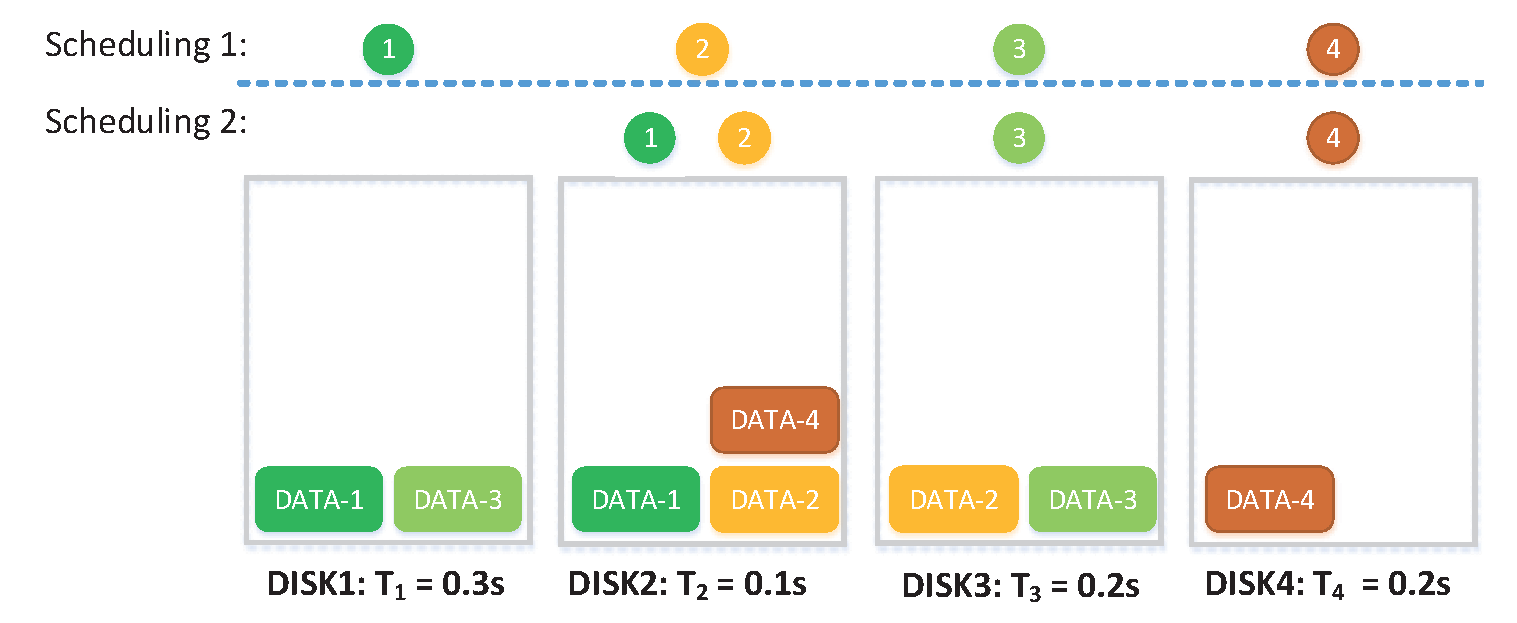
\includegraphics[height=1.4in]{fig1.eps}
	\caption{Comparison of task time between general task scheduling and disk-aware task scheduling. Scheduling1 is unaware of disk $read-time$ and the completion time of all tasks is max\{$T_1 * N_1$, $T_2 * N_2$, $T_3 * N_3$,  $T_4 * N_4$ \} = max\{0.3*1, 0.1*1, 0.2*3, 0.2*1\}= 0.3. Scheduling2 is aware of disk read time and the completion time of all tasks is max\{0, 0.1*2, 0.2*1, 0.2*1\} = 0.2. Scheduling2 is the optimum. }
	\label{fig1}
\end{figure}

Example shows that when choosing the disk for a task, two things need to be considered: the first is the $read-time$ of a disk, and the second is the load of the disk. These two things are able to ensure that there are no bottlenecks during the task execution and the data processing can be accelerated.

\begin{table}[!t]
	\Large
	\centering
	\footnotesize
	\renewcommand\arraystretch{1.2}
	\caption{NOTATIONS USED IN THIS PAPER.}
	\label{table-notations}
	\begin{tabular}{c|l}
		\hline
		$\mathbb{D}$ & \tabincell{l}{The set of heterogeneous disks in datacenter} \\
		\hline
		$\mathcal{M}$ & \tabincell{l}{The set of data in datacenter} \\
		\hline
		$\mathbb{T}$ & \tabincell{l}{The set of tasks to be scheduled} \\
		\hline
		$d_{i}$ & \tabincell{l}{The disk $i$ and $d_i \in \mathbb{D}$ } \\
		\hline
		$t_{j}$ & \tabincell{l}{The task $j$ and $t_j \in \mathbb{T}$ } \\
		\hline
		$m_{l}$ & \tabincell{l}{The data $l$ and $m_j \in \mathbb{M}$ } \\
		\hline
		$r_{l}^{k}$ & \tabincell{l}{The data replica $k$ of data  $m_l $ } \\
		\hline
		$read-time$ & \tabincell{l}{This time of reading a data block from disk } \\
		\hline
		$T_{i}$ & \tabincell{l}{The read-time of disk $d_i$} \\
		\hline	
		${I}_i^j$ & \tabincell{l}{A binary variable indicating if task $t_{i}$ choose the replica \\ that stored in $d_{i}$ as input  or not}\\
		\hline
		$\phi(t_j)$ & The data that task $t_j$ needs, and $\phi(t_j)$ $\in$  $\mathcal{M}$ \\
		\hline
		$\pi_{l}^{i}$ & \tabincell{l}{A binary variable indicating if data $m_l$ are \\stored at disk $d_i$ or not} \\
		\hline
		$h_{ul}$, $h_{dl}$ & \tabincell{l}{the channel fading coefficient for uplink and downlink} \\
		\hline
		$\phi(t_j)$ & The data that task $t_j$ needs \\
		\hline
		$N_(i)$ & Number of tasks which select data from disk i as input \\
		\hline
		$\tau$ & Size of each data replica in datacenter \\
		\hline
		$C$ & The number of replicas of each data. \\
		\hline
	\end{tabular}
\end{table}

\subsection{System Model}

The notations we need are shown in the table \ref{table-notations}. The data center is equipped with heterogeneous disks, and $\mathbb{D}$ is used to represent the set of all disks which are $d_{1}$, $d_{2}$, ...,$d_{|D|}$.  $\mathcal{M}$ denotes the set of all the data in data center, and each data is represented by $m_{1}$, $m_{2}$, ..., $m_{|M|}$. Each data $m_{l}$ has $C$ replicas which are $r_i^1$, $r_i^2$,... $r_i^{C}$ stored on $C$ different disks, with each data replica's size $\tau$, i.e. 64MB or 128MB. If the disk $d_{i}$ contains a replica of the data $m_l$, $\pi_l^{i}$ = 1. Otherwise, $\pi_l^{i}$ = 0. In datacenter with heterogeneous disks, each disk has its own $read-time$ represented by $T_i$, and the value of $T_i$ represents the time required to read a data replica from disk $t_i$.

When the query job arrives, the job will be divided into parallel tasks. $\mathbb{T}$ denotes the set of all tasks which include \{$t_1$, $t_2$, ..., $t_{T}$ \}. Each task $t_j$ corresponds to a unique input data $\phi(t_j)$. Since there are $C$ replicas of each data deployed in $C$ disks, the replicas of $\phi(t_j)$ exists in $C$ disks, assuming that it is $d_{j1}$, $d_{j2}$,... $d_{j|C|}$. So $t_j$ can read $\phi(t_j)$ from one of $C$ disks.

Next, if the task $t_j$ chooses the replica of data $\phi(t_j)$ stored in disk $d_i$, then $I_i^j$ = 1. In this case, the time of task $t_j$ reading the replica from disk $d_{j}$ is $I_i^j*T_i$. There may be some other tasks that select replicas stored in disk $d_{i}$, so the load of disk $d_{i}$ is $\sum_{j}I_i^j*T_i$. In order to avoid a large number of tasks to choose the same disk, resulting in data processing bottlenecks. Our objective is to minimize the maximum disk load.

\subsection{Heterogeneous Storage-aware Task Scheduling Problem Formulation ($\rm{HTS}$)} \label{HTS}

%$\mathcal{AP} \mathbb{AP}$ (~/~)

A large number of tasks are running in the cluster of data centers. If the scheduler are unaware of the heterogeneity of disks, it is likely that there are a large number of tasks that read data from the same low-speed disk, resulting in bottlenecks. To avoid this situation, we propose heterogeneous storage-aware task scheduling(HTS), as shown below. The optimization goal is to minimize the maximum disk load. Finally, by determining the value of the decision variable $I_i^j$, the appropriate disk is selected for each tasks to read the corresponding data. Detailed description is as follows:
\begin{align}
Min:&\;\;\;\;\;\max\limits_{i}\{\sum_{j}I_i^j*T_i\}\;[\rm{HTS}]\nonumber\\
s.t. 
&\;\;\;\;\;\sum_{i}I_i^j = 1,\;for\;\forall j\label{task-cons}\\
&\;\;\;\;\;I_i^j \leq \pi_{\phi(t_j)}^{d_i},\;for\;\forall i,j\label{data-cons}\\
&\;\;\;\;\;I_i^j\in\{0,1\},\;for\;\forall i,j\label{def-cons}
\end{align}

Constraint (\ref{task-cons}) indicates that task $t_j$ can only select one disk to read data $\phi(t_j)$. Constraint (\ref{data-cons}) indicates task $t_j$ can only read its input data from the disks which stores its input data. If one replica of data $\phi(t_j)$ is stored in disk $d_i$, then $\pi_{\phi(t_j)}^{d_i}$ = 1, otherwise $\pi_{\phi(t_j)}^{d_i}$ = 0. Constraint 3 denotes the range of decision variables, which can only be 0 or 1. $I_i^j$ = 1 indicates that task $t_j$ selects the replica stored on disk $d_i$ as input, while task $t_j$ = 0 is on the contrary.

The key to solve HTS problem is to determine the value of decision variables {$I_i^j$}. Next, we analyze the hardness of this problem and prove that the HTS problem is NP-hard. HTS problem can be reduced from the integer linear programming (ILP) problem. The ILP problem is NP-hard, and it follows that HTS problem is NP-hard. The specific proof process is as follows.

\emph{Theorem 1:} The HTS problem is NP-hard.

\emph{Proof:}
The canonical form \cite{b11} of ILP is described below.

For $m\times n$ matrix \textbf{A}
\begin{align}
Min:&\;\;\;\;\;\textbf{c}^T\textbf{x}\;\;[\rm{ILP}]\label{ILP}\\
s.t. 
&\;\;\;\;\;\textbf{A}\textbf{x}\geq \textbf{b}\nonumber\\
&\;\;\;\;\;\textbf{x} \geq0,\nonumber\\ 
and
&\;\;\;\;\;\textbf{x} \in \mathbb{Z}^n\nonumber
\end{align}

Taking the special case of HTS problem, the parameters are set as follows:
\begin{itemize}
	\item $\mathbb{D}$ = \{$d_0$, $d_1$, $d_2$\};$T_0$ = 1, $T_1$ = 1, $T_2$=1; $\mathbb{M}$ = \{$m_0$, $m_1$, ..., $m_{n-1}$\}; $C$ = 3
	\item $T$ = \{$t_0$, $t_1$, ..., $t_{n-1}$\}
\end{itemize}

It means that there are 3 disks, $d_0$, $d_1$, $d_2$, in the data center, each disk with a $read-time$ of 1. A total of n data, and each data has three replicas which deployed in the three disks, respectively. When the query job arrives, the job is divided into n tasks, $t_0$, $t_1$, ..., $t_n$ to read n data,$m_0$, $m_1$, ..., $m_n$, respectively.

For this particular case, the problem description can be modified to:

\begin{align}
Min:&\;\;\;\;\;\max\{\sum_{j}I_0^j, \sum_{j}I_1^j, \sum_{j}I_2^j\}\;[\rm{HTS-sp}]\\
s.t. 
&\;\;\;\;\;I_0^j + I_1^j +I_2^j= 1,\;for\;\forall j\nonumber\\
&\;\;\;\;\;I_0^j, I_1^j, I_2^j\in\{0,1\},\;for\;\forall j \in[0,n)\nonumber
\end{align}

Let  $x$ = $\sum_{j}I_0^j$, $y$ = $\sum_{j}I_1^j$, $z$ = $\sum_{j}I_2^j$, and the problem description can be modified to:
\begin{align}
Min:&\;\;\;\;\;\max\{x,y,z\}\;[\rm{HTS-sp}]\\
s.t. 
&\;\;\;\;\;x + y + z = n\;\label{enlarge-cons}\\
&\;\;\;\;\;0 \leq x, y, z \leq n  \;\;x, y, z\in\mathbb{Z}\nonumber
%&\;\;\;\;\;0 \leq y \leq n, y\in\mathbb{Z}\nonumber\\
%&\;\;\;\;\;0 \leq z \leq n, z\in\mathbb{Z}\nonumber
\end{align}
In the minimization problem, x + y + z = n can be modified to x + y + z = n and let $R$ denotes $\max\{x,y,z\}$. 

Finally, HTS-sp problem is converted to:
\begin{align}
Min:&\;\;\;\;\;0*x+0*y+0*z+R\;[\rm{HTS-ILP}]\label{HTS-ILP}\\
s.t. 
&\;\;\;\;\;x + y + z \geq n\;\nonumber\\
&\;\;\;\;\;-x + R \geq 0 \nonumber\\
&\;\;\;\;\;-y + R \geq 0  \nonumber\\
&\;\;\;\;\;-z + R \geq 0 \nonumber\\
&\;\;\;\;\;0 \leq x, y, z \leq n  \;\;x, y, z\in\mathbb{Z}\nonumber\\
%&\;\;\;\;\;0 \leq x \leq n, x\in\mathbb{Z}\nonumber\\
%&\;\;\;\;\;0 \leq y \leq n, y\in\mathbb{Z}\nonumber\\
%&\;\;\;\;\;0 \leq z \leq n, z\in\mathbb{Z}\nonumber\\
&\;\;\;\;\;R \geq 0, R\in\mathbb{Z}\nonumber
\end{align}

Obviously, HTS-ILP in (\ref{HTS-ILP}) is an instance of ILP in (\ref{ILP}). The decision version of 0-1 ILP (A variation in which only the restrictions must be satisfied, without optimization) is one of Karp's 21 NP-complete problems  \cite{b9}, so ILP is NP-hard. Further, the HTS-ILP problem is NP-hard.

On the one hand, when the optimal solution of HTS-ILP problem is obtained, the corresponding {x, y, z} can be converted into variable {$I_i^j$} in polynomial time by setting the value in \{$I_0^0$, $I_0^1$, ...,$I_0^{x-1}$, $I_1^{x}$, $I_1^{x+1}$, ..., $I_1^{x+y-1}$, $I_2^{x+y}$, $I_1^{x+y+1}$, ..., $I_2^{x+y+z-1}$\} to be 1, which will make the corresponding HTS-sp problem obtain the optimal solution. On the other hand, when the variable \{$I_i^j$\} make the HTS-sp problem obtain the optimal solution, the HTS-ILP also obtains the optimal solution by setting $x$ = $\sum_{j}I_0^j$, $y$ = $\sum_{j}I_1^j$, $z$ = $\sum_{j}I_2^j$. It can be seen from the above that any solution can be polynomially transformed between the HTS-sp and HTS-ILP. Therefore, HTS-sp is NP-hard. 

As a result of that HTS-sp is a special case in HTS, HTS problem is NP-hard.\hfill $\qedsymbol$

\section{DESIGN of ALGORITHMS FOR HTS PROBLEM}\label{DESIGN_ALGORITHM}

Due to the hardness of HTS problem, the optimal solution can not be obtained in polynomial time. In order to solve NP-hard problem, we propose a heuristic algorithm based on greedy idea, named HTS-greedy. However, this kind of algorithm usually has no guarantee of quality, although in some cases the solution is not bad, in some cases it is opposite. Furthermore, we design a quality assurance algorithm HTS-rdm, which makes the feasible solution approach to the optimal solution with probability 1- O($e^{-t^2}$) where t is the difference between the solution found by HTS-rdm and optimal solution.


\subsection{Heuristic Alogrithm}\label{Heuristic}

In this subsection, we will introduce the heuristic algorithm HTS-greedy specificly. Using the greedy idea, the HTS-greedy chooses the disk which stores $\phi(t_j)$ for each task $t_j$ and which has the minimum load, and finally outputs one disk for each task.


%Alogoritm1
\begin{algorithm}
	%\renewcommand{\thealgorithm}{}
	
	\textbf{Require:} For each task $t_j$, decide a disk $d_i$ that stores one replica of data $\phi(t_j)$.

	\begin{algorithmic}[1]
		\For{each disk $d_i$} \label{HTS-greedy:init}
			\State $load_{i}$ $\gets$ 0
		\EndFor
		\State Result $\gets$ \{\}
		\For{each task $t_j$} 
			\State $d_{j1}$, $d_{j2}$,... $d_{j|C|}$ = f($\phi(t_j)$)
		
			$//$Function f is a mapping from data to disks that stores each replica of the data.
			\State $load_{j_{min}}$ $\gets$ $\min\limits_{l}$($load_{j_l}$)
			
			$load_{j_{min}}$ $\gets$ $load_{j_{min}}$ + $T_{j_{min}}$
			\State Result $\gets$ Result $\cup$
			\{$\left \langle t_j, d_{j_{min}}\right \rangle$\}
		\EndFor
	
	\State \textbf{Return} Result
	\end{algorithmic}
	\caption{HTS-greedy}\label{HTS-greedy}
\end{algorithm}

Algorithm \ref{HTS-greedy:init} shows the detailed of HTS-greedy. Line 1-4 initializes $load_i$ = 0 and Result = \{\}, and $load_i$ denotes the total $read-time$ of the $disk_i$. Line 5-9 is to select a disk for each task $t_j$. In line 6, function f is used to help task $t_j$ find all disks that store replicas of data $\phi(t_j)$. Let $d_{j1}$, $d_{j2}$,... $d_{j|C|}$ denote the $C$ disks. Next, in line 7, the disk with minimum total $read-time$ is selected from the $C$ disks, and the $read-time$ caused by task $t_j$ is added to the $load_i$. Then put the task $t_j$ and disk $d_{j_l}$ into the set Result. After one iteration, the algorithm completes the decision for a task and it needs $\mathbb{T}$ iteration in total.

Next, an example is given to illustrate the algorithm. In datacenter, there exits a set of heterogeneous disks $\mathbb{D}$= \{$d_1$, $d_2$, $d_3$, $d_4$\} with $read-time$ $T_1$ = 0.3,  $T_2$ = 0.1,  $T_3$ =0.2 and $T_4$ =0.2, respectively. Data set $\mathbb{M}$ = \{$m_1$, $m_2$, $m_3$, $m_4$\} are stored as Fig.\ref{fig1}. Obviously, each data has two replicas. When query tasks $\mathbb{T}$= \{$t_1$, $t_2$, $t_3$, $t_4$\} ($\phi(t_j)$ = j, 1 $\leq$j$ \leq$ 4) comes, the algorithm HTS-greedy runs as follows: %($\phi(t_j)$ = j (1 $\leq$j$ \leq$ 4, task $t_j$'s input is $m_j$ which equals the DATA-j in Fig.\ref{fig1}))

Initial: Reslut = \{\}, $load_1$=0, $load_2$=0, $load_3$=0, $load_4$=0
\begin{itemize}
	\item \textbf{Round 1}:for task  $t_1$:
	 f($\phi(t_1)$) = \{1, 2\} = \{DISK1, DISK2\}\\
	 $load_1$ = $\min$\{$load_1$ = 0, $load_2$ = 0\}\\
	 $load_1$ = $load_1$ + $T_1$ = 0.3\\
	Result = Result $\cup$ $\left \langle t_1, d_{1}\right \rangle$ = \{$\left \langle t_1, d_{1}\right \rangle$\}
	\item \textbf{Round 2}:for task  $t_2$:
	f($\phi(t_2)$) = \{2, 3\}\\
	$load_2$ = $\min$\{$load_2$ = 0, $load_3$ = 0\}\\
	$load_2$ = $load_2$ + $T_2$ = 0.1\\
	Result = Result $\cup$ $\left \langle t_2, d_{2}\right \rangle$ = \{$\left \langle t_1, d_{1}\right \rangle$, $\left \langle t_2, d_{2}\right \rangle$\}
	\item \textbf{Round 3}:for task  $t_3$:
	f($\phi(t_3)$) = \{1, 3\}\\
	$load_3$ = $\min$\{$load_1$ = 0.3, $load_3$ = 0\}\\
	$load_3$ = $load_3$ + $T_3$ = 0.2\\
	Result = Result $\cup$ $\left \langle t_3, d_{3}\right \rangle$ = \{$\left \langle t_1, d_{1}\right \rangle$, $\left \langle t_2, d_{2}\right \rangle$,  $\left \langle t_3, d_{3}\right \rangle$\}
	\item \textbf{Round 4}:for task  $t_4$:
	f($\phi(t_4)$) = \{2, 4\}\\
	$load_4$ = $\min$\{$load_2$ = 0.1, $load_4$ = 0\}\\
	$load_4$ = $load_4$ + $T_4$ = 0.2\\
	Result = Result $\cup$ $\left \langle t_4, d_{4}\right \rangle$ = \{$\left \langle t_1, d_{1}\right \rangle$, $\left \langle t_2, d_{2}\right \rangle$,  $\left \langle t_3, d_{3}\right \rangle$, $\left \langle t_4, d_{4}\right \rangle$\}
	
\end{itemize}

\begin{figure}[!t]
	\centering
	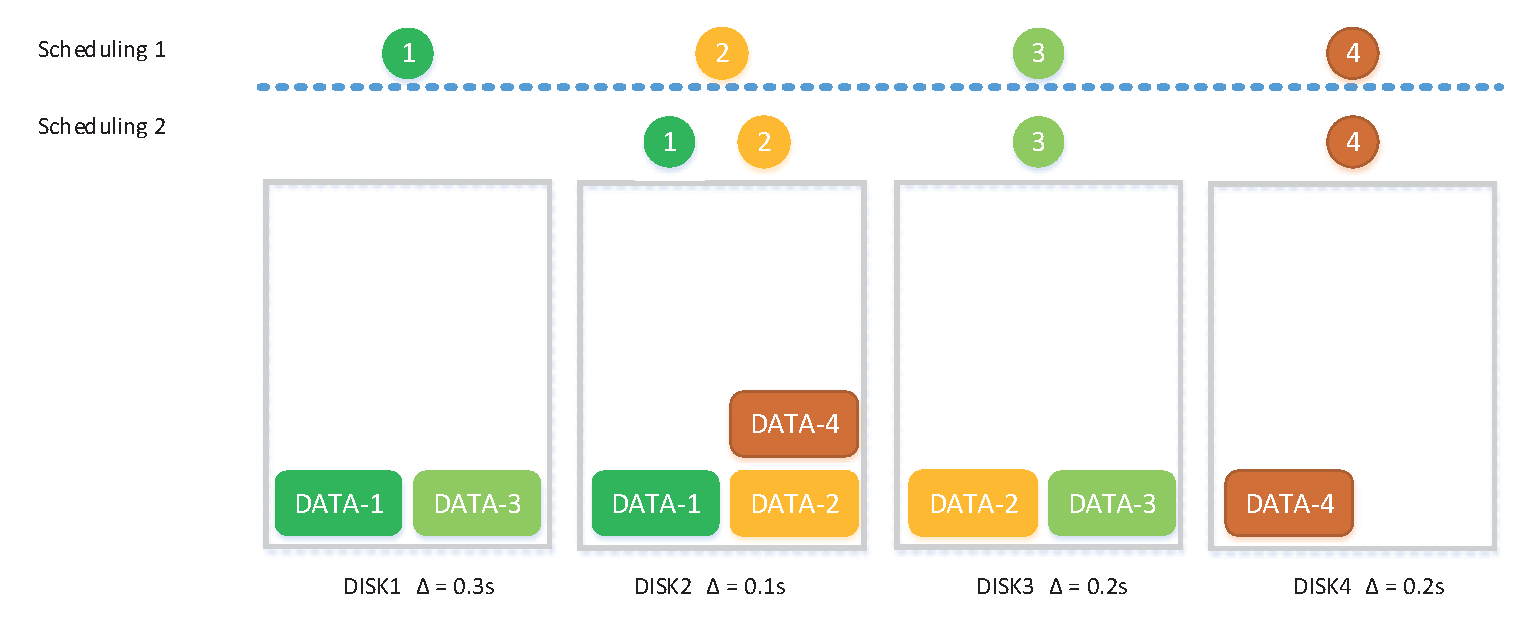
\includegraphics[height=0.8in]{fig2.eps}
	\caption{The process of algorithm HTS-greedy execution for the input in Fig.\ref{fig1}. }
	\label{fig2}
\end{figure}

The final result is in Result and  Tasks will follow \{$\left \langle t_1, d_{1}\right \rangle$, $\left \langle t_2, d_{2}\right \rangle$,  $\left \langle t_3, d_{3}\right \rangle$, $\left \langle t_4, d_{4}\right \rangle$\} to read data.The specific process of HTS-greedy algorithm is shown in Fig.\ref{fig2}.

\subsection{Randomized Alogrithm}\label{Randomized}

In the previous section \ref{Heuristic}, we designed a greedy heuristic algorithm HTS-greedy to solve HTS problems. However, this algorithm does not have performance guarantee. Therefore, in this subsection, we propose a performance-guaranteed random algorithm HTS-rdm. By relaxing the HTS problem to HTS-relaxation problem, HTS-rdm uses linear programming to solve HTS-relaxation. The decomposition obtained by linear programming is a fraction rather than an integer, which represents the preference when selecting disks. Subsequently, we prove that the solution found by the HTS-rdm algorithm can approach the optimal solution with probability 1- O($e^{-t^2}$) where t is the difference between the solution found by HTS-rdm and optimal solution..

\paragraph{\textbf{Relaxation of HTS Problem}} According to the previous analysis \ref{HTS}, this problem is NP-hard, which cannot be solved in polynomial time. But the linear programming (LP) problem is solvable in polynomial time, a natural point of view is to relax the HTS problem to LP. The method is to change the range of variables from integer domain \{0, 1\} to real domain [0, 1]. As shown below, HTS-relaxtion, this process is named \textbf{relaxation}. The solution of HTS-relaxtion provides a lower bound for the original HTS problem (HTS is a minimization problem. For the maximization problem is on the contrary). Next, based on the solution of linear programming, the fractional solution is mapped back to integer in some way, which is named \textbf{rounding}. Based on relaxation-rounding, we propose HTS-rdm algorithm.

 \begin{align}
 Min:&\;\;\;\;\;\max\limits_{i}\{\sum_{j}p_i^j*T_i\}\;[\rm{HTS-relaxtion}]\nonumber\\
 s.t. 
 &\;\;\;\;\;\sum_{i}p_i^j = 1,\;for\;\forall j\nonumber\\
 &\;\;\;\;\;p_i^j \leq \pi_{\phi(t_j)}^{d_i},\;for\;\forall i,j\nonumber\\
 &\;\;\;\;\;p_i^j \in[0, 1],\;for\;\forall i,j\nonumber
 \end{align}
 
 The detailed procedure of HTS-rdm algorithm is shown in Algorithm \ref{HTS-rdm}. Line 1 initializes the Result set, which stores the final result. In the second line, the HTS-relaxation problem is solved by linear programming tools. The third line uses rounding strategy to convert fractional solution to integer solution. Line 4-9 organize the results and output them. Then the task will read the disk according to the results. The specific rounding strategies are as follows:
 
 The value of \{$p_i^j$\}  $\in$ [0, 1] which shows the correlation between task $t_j$ and disk $d_i$. Therefore, we can select disk $d_i$ for task $t_j$ with  probability \{$p_i^j$\}. The method is to use the parameter $q_j$, which is randomly selected in (0,1]. If the $q_j$ $\in$ ($\sum p_{r-1}^{j}$, $\sum p_{r}^{j}$], then $I_r^j = 1$, otherwise, $I_i^j$ = 0 ($\forall$ $i$, $i \ne r$). This approach ensures only one disk can be selected for each task.%For each task $t_j$, the corresponding decision variables are \{$p_0^j$,$p_i^j$, ..., $p_i^j$\}. 
 \begin{algorithm}
 	%\renewcommand{\thealgorithm}{}
 	
 	\textbf{Require:} Decide a disk $d_i$ for each task $t_j$. %and $d_i$ stores data $\phi(t_j)$.
 	\begin{algorithmic}[1]
 		
 		\State Result $\gets$ \{\}
 		\State \{$p_i^j$\} = HTS-relaxtion		
 		$//$ is the solution of HTS-relaxtion problem. 
 		
 		\State Based on \{$p_i^j$\}, use rounding strategy and get \{$I_i^j$\}
 		\For{$\forall$ $i$, $j$}  
 			\If{$I_i^j$ == 1}
 			\State Result $\gets$ Result $\cup$ 	
 			\{$\left \langle t_j, d_i\right \rangle$\}
 			\EndIf
 		\EndFor	
 		\State \textbf{Return} Result	
 	\end{algorithmic}
 	\caption{HTS-rdm}\label{HTS-rdm}
 \end{algorithm}

\paragraph{\textbf{Analysis of HTS-rdm Algorithm}}

In this section, we will prove that the HTS-rdm algorithm can approach the optimal solution with a probability 1- O($e^{-t^2}$). Firstly, we prove that the difference between $read-time$ contributed by any tasks $t_j$ to $d_i$ and expectation is matingales sequence \cite{b12}. Secondly, Based on the matigales sequence, we use Azuma inequality to illustrate the bound between the feasible solution and the optimal solution.
\begin{figure*}[!t]
	\centering
	\subfigure[Small Workload ]{\label{Fig:instance1}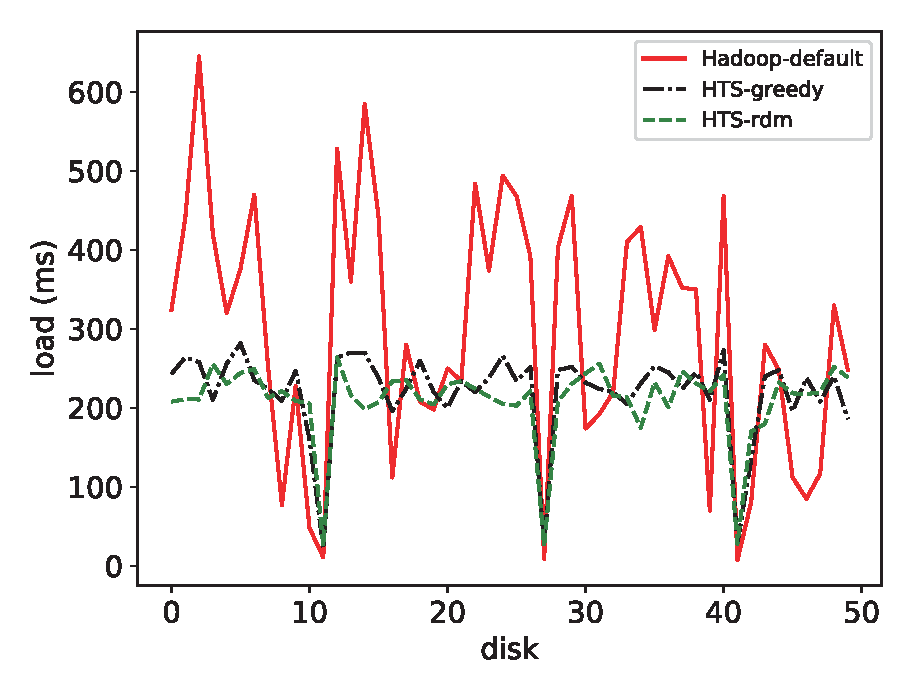
\includegraphics[height=1.6in]{fig_instance1_1.eps}}\quad\quad %quad 表示图像的间距
	\subfigure[Medium Workload ]{\label{Fig:instance2}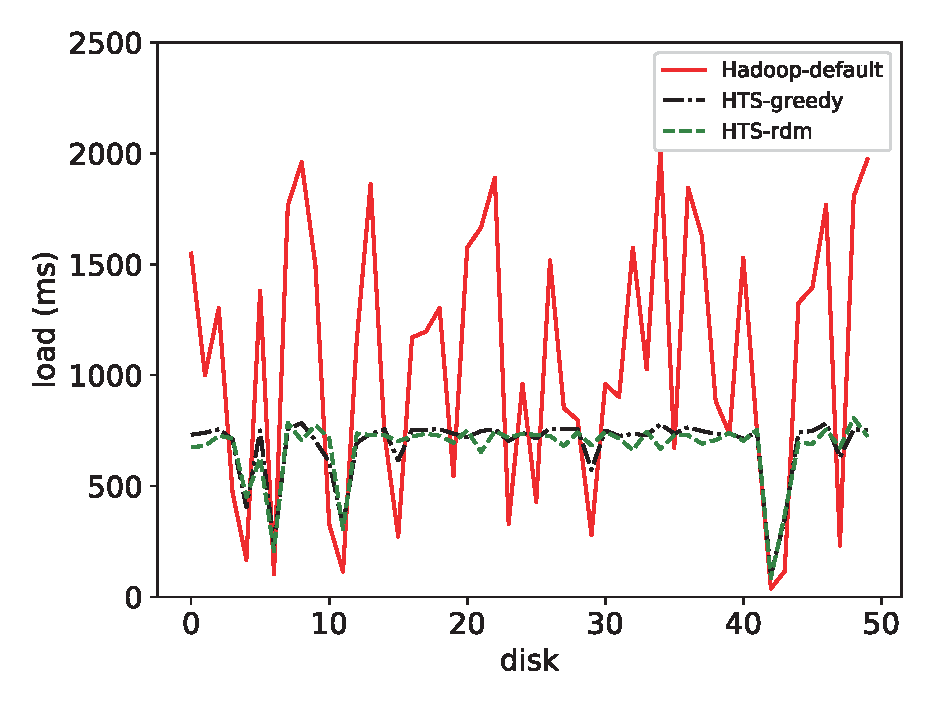
\includegraphics[height=1.6in]{fig_instance2_2.eps}}\quad\quad
	\subfigure[Large Workload
	]{\label{Fig:instance3}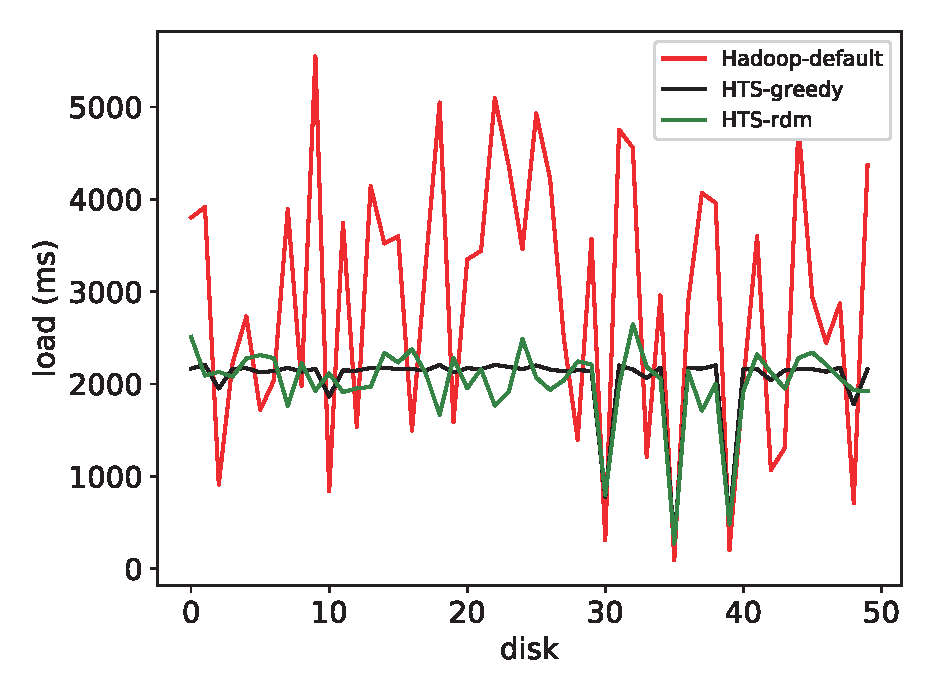
\includegraphics[height=1.6in]{fig_instance3_1.eps}}
	\vspace{-1ex}
	\caption{Comparison of HTS-rdm and other Algorithm on different Workloads. \ref{Fig:instance1} denotes the results on Small Workload which has about 500 tasks. \ref{Fig:instance2} denotes the results on Medium Workload which has about 2000 tasks.
	\ref{Fig:instance3} denotes the results on Large Workload which has 5000 tasks. X-axis denotes the disk. Y-axis denotes the load of each disk after running the three algorithms.}
	\label{Fig:instance}
	\vspace{-1ex}
\end{figure*}


\emph{Theorem 2:} Pr[SOL(HTS-rdm) - OPT(HTS) $\leq$ t] $\geq$ 1 - O($e^{-t^2}$).

\emph{Proof:}

SOL(HTS-rdm) denotes the feasible solution found by HTS-rdm algorithm and  OPT(HTS) denotes the optimum solution of HTS problem.

Firstly, task $t_j$'s contribution to disk $d_i$'s load is expressed as:
 \begin{align}
&\;\;\;\;\;Z_i^j = I_i^j*T_i
\end{align}

From the rounding strategy in Algorithm \ref{HTS-rdm}, we can get that:
 \begin{align}
&\;\;\;\;\;Pr[I_i^j = 1] = p_i^j,\;\;for\forall i,j \nonumber
\end{align}
%Therefore

The expectation of $Z_i^j$ is
\begin{align}
E[Z_i^j] &\;\;\;= E[I_i^j]*T_i \nonumber\\
&\;\;\;= (Pr[I_i^j = 1] * 1 + Pr[I_i^j = 0] * 0)*T_i \nonumber\\
&\;\;\;= p_i^j*T_i\label{prove:expect}
\end{align}

The difference between $Z_i^j$ and $E[Z_i^j]$ defines as
\begin{align}
Q_i^j = Z_i^j - E[Z_i^j]\label{prove:diff}
\end{align}

For the all $\mathbb{|T|}$ tasks, $L_i^{\mathbb{|T|}}$ denotes the sum of $Q_i^j$ in disk $d_i$:
\begin{align}
L_i^{\mathbb{|T|}} = \sum_{j = 1}^{\mathbb{|T|}} Q_i^j
= \sum_{j = 1}^{\mathbb{|T|} - 1} L_i^j + Q_i^{\mathbb{|T|}} \label{prove:L_margin}
\end{align}
Then, on the condition $L_i^{1}$, $L_i^{2}$, ..., $L_i^{r-1}$, the expectation of $L_i^{r}$ is:
\begin{align}
&E[L_i^{r}|L_i^{1}, L_i^{2}, ..., L_i^{r-1}] \nonumber\\
&\overset{\text{(\ref{prove:L_margin})}}{=}E[L_i^{r-1} + Q_i^{r} |L_i^{1}, L_i^{2}, ..., L_i^{r-1}] \nonumber\\
&\overset{\text{}}{=}E[L_i^{r-1} |L_i^{1}, L_i^{2}, ..., L_i^{r-1}]
+ E[Q_i^{r} |L_i^{1}, L_i^{2}, ..., L_i^{r-1}] \nonumber\\
&\overset{\text{(\ref{prove:diff})}}{=}L_i^{r-1} + E[Z_i^r - E[Z_i^r] |L_i^{1}, L_i^{2}, ..., L_i^{r-1}]\nonumber\\
&=L_i^{r-1} + E[Z_i^r|L_i^{1}, L_i^{2}, ..., L_i^{r-1}]
-E[E[Z_i^r] |L_i^{1}, L_i^{2}, ..., L_i^{r-1}]\nonumber\\
&=L_i^{r-1} + E[Z_i^r] - E[Z_i^r]\nonumber\\
&=L_i^{r-1}\label{prove:marginsq}
\end{align}
Therefore, $L_i^{1}$, $L_i^{2}$, ..., $L_i^{|\mathbb{T}|}$ are matigales sequence \cite{b13}. For completeness, we let $L_i^{0}$ = 0. And for $\forall r \geq 1$, we have:
\begin{align}
  |L_i^r - L_i^{r-1}|\overset{\text{(\ref{prove:L_margin})}}{=} |Q_i^{r}| \overset{\text{(\ref{prove:diff})}}{=} |Z_i^j - E[Z_i^j]|\leq g_i^r\\
  g_i^r = \max\{T_i -  E[Z_i^j], E[Z_i^j]\}\label{prove:bound}
\end{align}

From above (\ref{prove:bound}), any two adjacent values $L_i^r$, $L_i^{r-1}$ in the margingales sequence have constant bounds $g_i^r$. Based on (\ref{prove:marginsq}) and (\ref{prove:bound}), we can use Azuma's inequality. Then, 

\begin{align}
Pr\{L_i^{|\mathbb{T}|} - L_i^{0} \geq t\} \leq exp\{-\frac{t^2}{2\sum_{ i = 1 }^{|\mathbb{T}|}(g_i^k)^2}\} \label{prove:azuma}
\end{align}

Substitute equations (\ref{prove:diff}) and (\ref{prove:L_margin}) into the upper equation (\ref{prove:azuma}). Then, 

\begin{align}
Pr\{\sum_{j = 1}^{|\mathbb{T}|} Z_i^j - 
	\sum_{j = 1}^{|\mathbb{T}|} E[Z_i^j]\geq t\} \leq exp\{-\frac{t^2}{2\sum_{ i = 1 }^{|\mathbb{T}|}(g_i^k)^2}\} \label{prove:azuma1}
\end{align}
 The (\ref{prove:azuma1}) is equal to:
\begin{align}
Pr\{\sum_{j = 1}^{|\mathbb{T}|} Z_i^j \leq \sum_{j = 1}^{|\mathbb{T}|} E[Z_i^j] + t\} \geq 1 - exp\{-\frac{t^2}{2\sum_{ i = 1 }^{|\mathbb{T}|}(g_i^k)^2}\}\nonumber\\
= 1 - O(e^{-t^2})\label{prove:azuma3}
\end{align}

Let $S_i$  = $\sum_{j = 1}^{|\mathbb{T}|} Z_i^j$,
$E_i$ = $\sum_{j = 1}^{|\mathbb{T}|} E[Z_i^j]$
$\overset{\text{(\ref{prove:expect})}}{=}$
$\sum_{j = 1}^{|\mathbb{T}|} p_i^j*T_i$. Then,
\begin{align}
Pr\{S_i \leq U_i + t\} \geq 1- O(e^{-t^2}) \label{prove:SU}
\end{align}

$S_i$ denotes the load of disk $d_i$ which is the result of ILP. And $E_i$ denotes the expectation which is the result of LP. Because LP provides a lower bound for the optimal solution of ILP problem (HTS is a minimization problem. For the maximization problem is on the contrary), we have:



\begin{align}
E_i \leq OPT(HTS)\label{prove:OPT}
\end{align}

Take $S_u$, $E_v$ as
\begin{align}
	S_u = S_{max} = \max_i S_i\\
	E_v = E_{max} = \max_i E_i\label{prove:Emax}
\end{align}

Then, we have the following inequalities,
\begin{align}
SOL(HTS-rdm) = S_u  
\overset{\text{(\ref{prove:azuma3})}}{\leq}  E_u+t
\overset{\text{(\ref{prove:Emax})}}{\leq} E_v+t\nonumber\\
\overset{\text{(\ref{prove:OPT})}}{\leq} OPT(HTS)+t\label{prove:SOL-OPT}
\end{align}

From (\ref{prove:SU}) and (\ref{prove:SOL-OPT}), we can conclude that,
\begin{align}
Pr\{SOL(HTS-rdm)<OPT (HTS)+t\} \geq 1 - O(e^{-t^2})\label{prove:result}
\end{align}

Observed from the (\ref{prove:result}), the feasible solution SOL(HTS-rdm) found by the algorithm and the optimal solution OPT (HTS) are approximated by probability $1 - O(e^{-t^2})$. When hundreds of tasks are deployed with $1 - O(e^{-t^2})$ = 0.85, the value of $t$ is acceptable, only a few millisecond.\hfill $\qedsymbol$


\section{PERFORMANCE EVALUATION}\label{PERFORMANCE_EVALUATION}

In this section, we implement our algorithms HTS-greedy and HTS-rdm, and compare our algorithms with storage-unaware scheduling algorithm. The results show that performance can be improved by 40\%.
\subsection{Simulation Settings}\label{SCM}
Usually, the general scheduling mechanism can not perceive the heterogeneity of the disk. For example, in Hadoop the scheduler cannot know the load of the disk when deploying the task. When selecting data replica for tasks, it is usually a random selection strategy, which we call Hadoop-default. We compare our proposed algorithms with it.

\textbf{Workload:} Referring to the characteristics of Google traces \cite{b20}, we classify workload into three categories: Small Workload, Medium Workload and Large Workload, as shown in TABLE \ref{tab:workload}. In Small Workload, most of the jobs have 1-150 tasks. In has Large Workload, there are 50\% of the jobs that has over 50 tasks. The Medium Workload is in the middle of them.

\begin{table}[htbp]
	\caption{THE DIFFERENT TRACES USED FOR EXPERIMENT}
	\begin{center}
		\begin{tabular}{|c|c|c|c|}
			\hline
			 \diagbox{Traces}{Number of tasks} & 1-150 & 150-500 & $\ge$ 500\\
			\hline
			Small Workload & 96\% & 2\% & 2\%\\
			\hline
			Medium Workload & 50\% & 40\% & 10\%\\
			\hline
			Large Workload & 40\% & 10\% & 50\%\\
			\hline
		\end{tabular}
		\label{tab:workload}
	\end{center}
\end{table}

\textbf{Setting:}
In distributed file systems \cite{b19}, data is distributed uniformly on disk. Therefore, in this experimental environment, we uniformly deploy 200000 data with three data replicas by default, each data block size $\tau$ = 128MB. 500 disks are set up by default. The $read-time$ of the disk in the cluster is between 10 and 500 in ms. 


\begin{figure*}[!t]
	\centering
	\subfigure[Results under varilous setting on Workloads ]{\label{Fig:completeWorkload}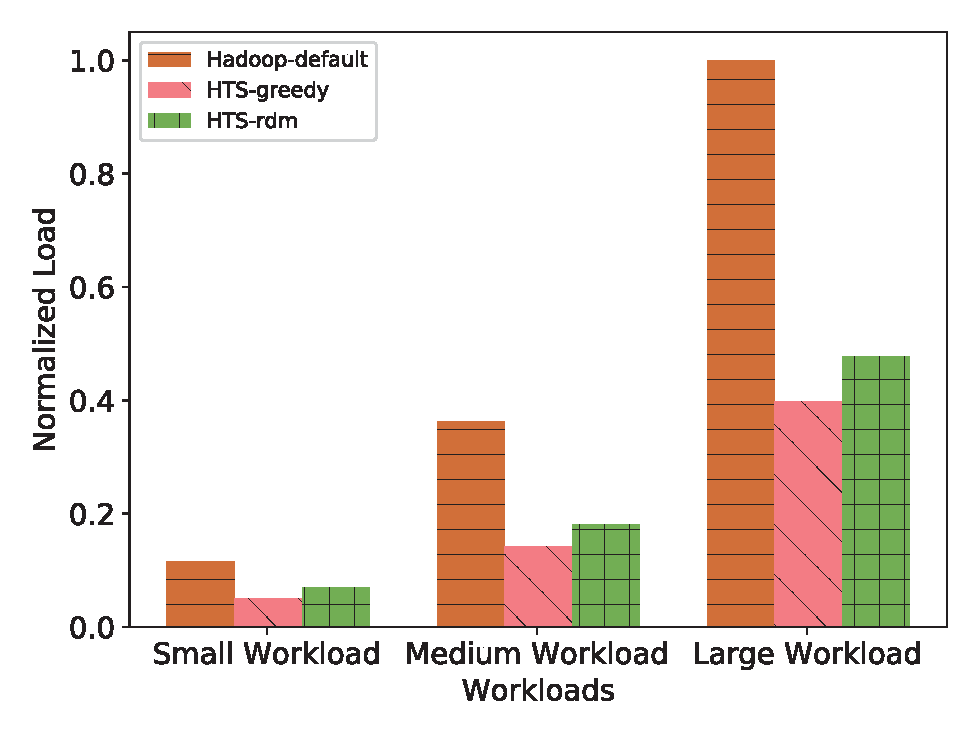
\includegraphics[height=1.6in]{figcomplete1_3.eps}}\quad\quad %quad 表示图像的间距
	\subfigure[Results under different Heterogeneity cluter. ]{\label{Fig:completeHeter}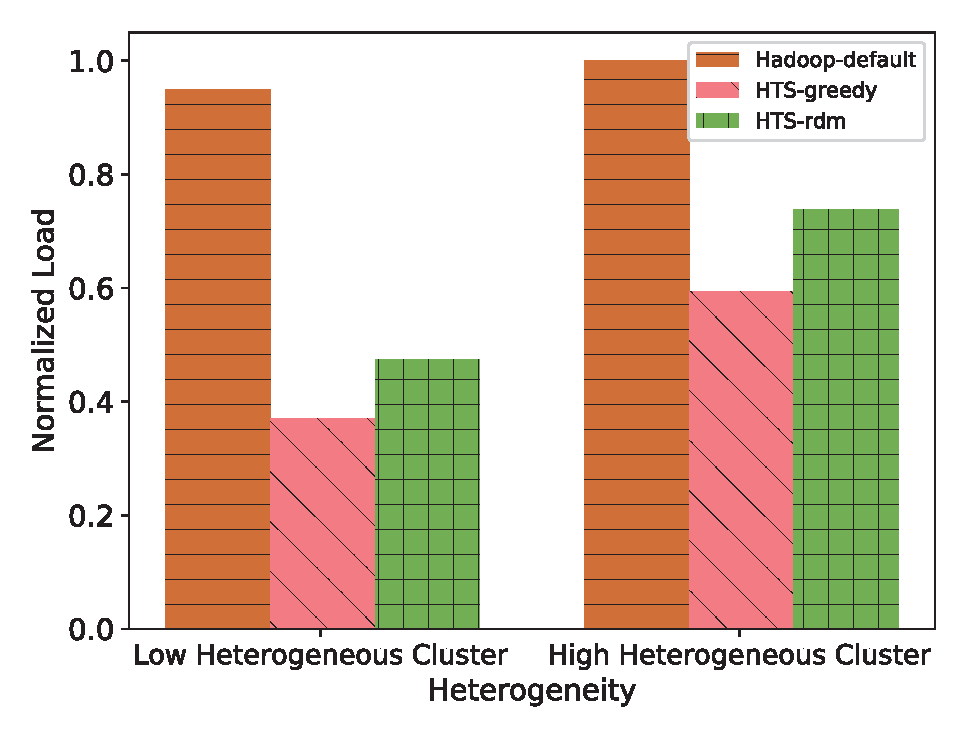
\includegraphics[height=1.6in]{figcomplete2_3.eps}}\quad\quad
	\subfigure[Results under varilous setting on reolicas number
	]{\label{Fig:completeRep}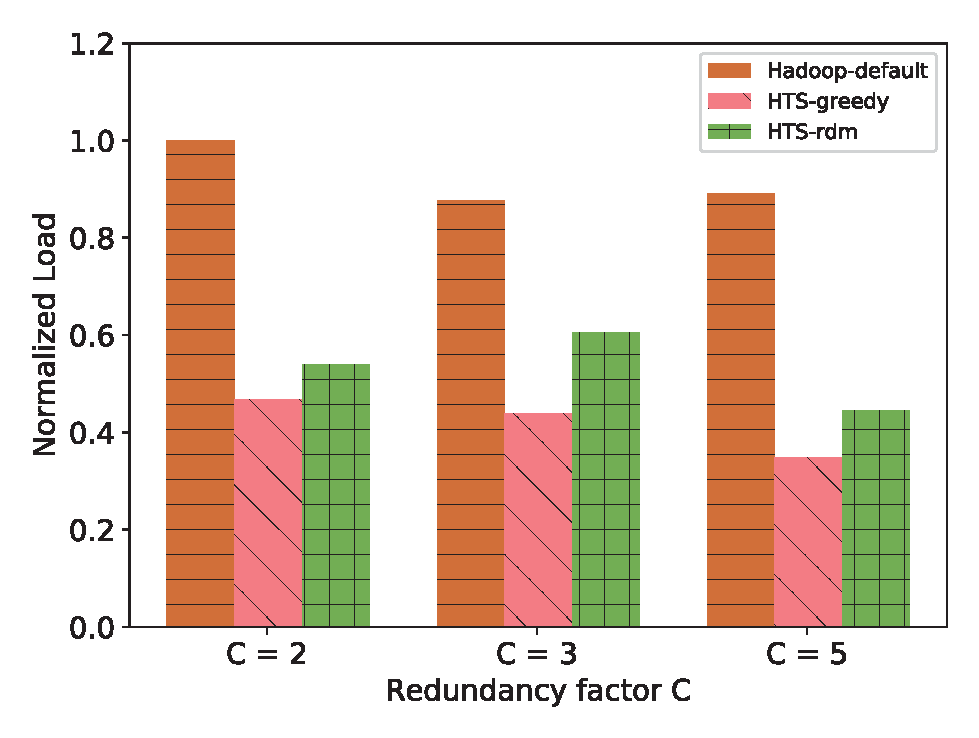
\includegraphics[height=1.6in]{figcomplete3_3.eps}}
	\vspace{-1ex}
	\caption{Comparison of HTS-rdm and other Algorithm on different workloads, different heterogenelity cluter and different replica number $C$. \ref{Fig:completeWorkload} denotes effect of different workloads on completion time. \ref{Fig:completeHeter} denotes the completion time of the three algorithm on different Heterogeneity cluter. \ref{Fig:completeRep} denotes the completion time of the three algorithm when $C$ is different. Y-axis denotes the completion time of all tasks which has been normalized.}
	\label{Fig:complete}
	\vspace{-3ex}
\end{figure*}

\subsection{Simulation Results}

For convenience of display, Fig.\ref{Fig:instance}. shows the results under different workloads upon 50 disks. X-axis denotes the disks. Y-axis denotes the load of each disk after running the three algorithms. The lower the peak of the curve, the better the result. The black dotted line represents the execution result of Algorithm HTS-greedy, and the green line represents the execution result of Algorithm HTS-rdm. Overall, we can see that our algorithm performs better than Hadoop-default. As shown in Fig.\ref{Fig:instance1}, in the small workload, the result of Hadoop-default has large fluctuations. This is because hadoop-default does not perceive the $read-time$ and load of the disk when selecting a replica for the task. Even if the tasks are deployed uniformly on disks, the disk with low performance may have a relatively large load. In Fig. \ref{Fig:instance1}, low performance disks will have high peaks. Completion of all parallel tasks is the end of the big data processing job. Therefore, the task reading data from the disk with poor performance will be the bottleneck of data processing job. For example, Hadoop-default causes the tasks of reading data from disk-2 to be the bottleneck of big data processing in the Fig.\ref{Fig:instance1} which is 654. Algorithms HTS-greedy and HTS-rdm can maintain roughly all disks at a lower load, less than 300. The reason is that HTS-greedy can select the disk to read for the task according to load of the disks and HTS-rdm can select the disk to read for the task according to load of the disks the performance of the disk. The maximum load of HTS-greedy algorithm is 261 in disk-12. Compared with the Hadoop-default, the performance is improved by 64\%. The maximum load of HTS-rdm algorithm is disk-4, and the corresponding load is 284. Compared with the baseline algorithm, the performance of HTS-rdm algorithm improves 57\%.
As the number of tasks increases, the load on all disks increases. For example, in Fig.\ref{Fig:instance2}, when the number of tasks is about 2000, in Hadoop-default algorithm the maximum load is 2009 in disk-9. The results of HTS-greedy and HTS-rdm are that 784 in disk-8  and 770 in disk-6, respectively. The performance of our algorithm improves by 61\% and 62\%. 
When the number of tasks becomes larger, in the large Workloads of Fig. \ref{Fig:instance3}, the maximum load obtained by the three algorithms are 5546,2205 and 2646. HTS-greedy increases by 60\% and HTS-rdm performance improves by 52\%.
 
Next, we study the impact of different factors workloads, degree of heterogeneity and the number of data replicas, on the load upon the default configuration. In Fig.\ref{Fig:completeWorkload}, the horizontal X-axis represents different workloads, and the Y-axis represents the maximum load in the cluster, which has been normalized. In the previous part, impact of Workloads is that the overall load on disk shows an increasing trend as the Workloads gets larger. Fig.\ref{Fig:completeWorkload} shows the difference among the three workloads. The performance of our proposed algorithm can always be improved by 60\% on average. Next, we observed the effect of degree of heterogeneity on the load. We divide the heterogeneity of the cluster into two kinds. One is that the $read-time$ of disks is evenly distributed between 10ms and 100ms, named Low Heterogeneous Cluster. Another is High Heterogeneous Cluster, where the $read-time$ of disks is evenly distributed between 10ms and 500ms. Other conditions are configured by default. From Fig.\ref{Fig:completeHeter}, when the degree of heterogeneity gets larger, the overall load shows an increasing trend. This is because the large the degree of heterogeneity, the greater the performance difference between disks. This leads to hard balancing of disk loads. Through \ref{Fig:completeHeter}, we find that our algorithm can also improve the performance of 40-50\% in clusters with high heterogeneity. Finally, we analyze the impact of the amount of data replicas on disk load. We set the number of data replicas as 2, 3 and 5. Observe that the higher the number of replicas, the lower the disk load. Reason for it is that with the number of data replicas increasing, the probability of data being deployed on high performance disks increases. Selecting data on high-performance disks at this time will greatly accelerate the completion of tasks. When $C$ = 5, our algorithm can achieve 65\% performance improvement.
 
 All in all,  the performance of the two algorithms proposed by us has reached an average of 55\% improvement over baseline algorithm on average under different conditions.



\section{CONCLUSION}\label{CONCLUSION}
There is a trend of more and more heterogeneous disks in data centers. Due to the heterogeneity, a mismatch occurred between the upper software  and the lower hardware, which leads to the low performance of big data analysis. To minimize the latency of big data analysis. Based on this, we first formulate the heterogeneous storage awareness task scheduling problem, and prove the hardness of the problem. Then we propose two effective algorithms, heuristic algorithm and quality assurance random algorithm, to solve this problem. Experiments show that our algorithm speeds up the average completion time by 55\%. 
\section*{Acknowledgment}
None





\begin{thebibliography}{00}
\bibitem{b1} Ahmad F, Chakradhar S T, Raghunathan A, et al. Tarazu: optimizing mapreduce on heterogeneous clusters[C]//ACM SIGARCH Computer Architecture News. ACM, 2012, 40(1): 61-74.
\bibitem{b2} Zaharia M, Borthakur D, Sen Sarma J, et al. Delay scheduling: a simple technique for achieving locality and fairness in cluster scheduling[C]//Proceedings of the 5th European conference on Computer systems. ACM, 2010: 265-278.
\bibitem{b3} Ananthanarayanan G, Agarwal S, Kandula S, et al. Scarlett: coping with skewed content popularity in mapreduce clusters[C]//Proceedings of the sixth conference on Computer systems. ACM, 2011: 287-300.
\bibitem{b4} Abad C L, Lu Y, Campbell R H. DARE: Adaptive data replication for efficient cluster scheduling[C]//2011 IEEE international conference on cluster computing. IEEE, 2011: 159-168.
\bibitem{b5} Jalaparti V, Bodik P, Menache I, et al. Network-aware scheduling for data-parallel jobs: Plan when you can[C]//ACM SIGCOMM Computer Communication Review. ACM, 2015, 45(4): 407-420.
\bibitem{b6} Xu L, Butt A R, Lim S H, et al. A heterogeneity-aware task scheduler for spark[C]//2018 IEEE International Conference on Cluster Computing (CLUSTER). IEEE, 2018: 245-256.
\bibitem{b7} Pan F, Xiong J, Shen Y, et al. H-Scheduler: Storage-Aware Task Scheduling for Heterogeneous-Storage Spark Clusters[C]//2018 IEEE 24th International Conference on Parallel and Distributed Systems (ICPADS). IEEE, 2018: 1-9.
\bibitem{b8} Wang B, Jiang J, Yang G. Actcap: Accelerating mapreduce on heterogeneous clusters with capability-aware data placement[C]//2015 IEEE Conference on Computer Communications (INFOCOM). IEEE, 2015: 1328-1336.
\bibitem{b9} Karp R M. Reducibility among combinatorial problems[M]//Complexity of computer computations. Springer, Boston, MA, 1972: 85-103.
\bibitem{b10} Hromkovič J. Algorithmics for hard problems: introduction to combinatorial optimization, randomization, approximation, and heuristics[M]. Springer Science \& Business Media, 2013.
\bibitem{b11} 2018. Integer programming. https://en.wikipedia.org/wiki/Integer\_programming.
\bibitem{b12} Grimmett G, Grimmett G R, Stirzaker D. Probability and random processes[M]. Oxford university press, 2001.
\bibitem{b13} 2019. Martingale (probability theory). https://en.wikipedia.org/wiki/Martingale\_(probability\_theory)

\bibitem{b14} Wang B, Jiang J, Yang G. Actcap: Accelerating mapreduce on heterogeneous clusters with capability-aware data placement[C]//2015 IEEE Conference on Computer Communications (INFOCOM). IEEE, 2015: 1328-1336.
\bibitem{b15} Apache Spark. https://spark.apache.org, 2019.
\bibitem{b16}Seagate. https://www.seagate.com/cn/zh/.
\bibitem{b17}Samsung. https://www.samsung.com/semiconductor/cn/, 2019.
\bibitem{b18}Guo Z, Fox G, Zhou M. Investigation of data locality in mapreduce[C]//Proceedings of the 2012 12th IEEE/ACM International Symposium on Cluster, Cloud and Grid Computing (ccgrid 2012). IEEE Computer Society, 2012: 419-426.
\bibitem{b19} Hdfs. https://hadoop.apache.org/hdfs, 2019.
\bibitem{b20} 2012. Google Cluster Trace. https://code.google.com/p/googleclusterdata/.

\bibitem{b25} F. Ahmad, S. Chakradhar A. Raghunathan and T. N. Vijaykumar. Tarazu: optimizing mapreduce on heterogeneous clusters. In ACM ASPLOS 2012.
\bibitem{b26} R. Gandhi, D. Xie, Y. Charlie. PIKACHU: How to Rebalance Load in Optimizing MapReduce On Heterogeneous Clusters. In USENIX ATC 2013.

\end{thebibliography}
\end{document}

